\begin{lstlisting}
Section 6.5:  4,  5(b),   6,  7;   
6(b): This Λ is a function of what F-statistic that would actually be used in this test?  
Section 7.1:  2,  4,  5,  8
\end{lstlisting}
\begin{exercise}
\begin{figure}[H]
\centering
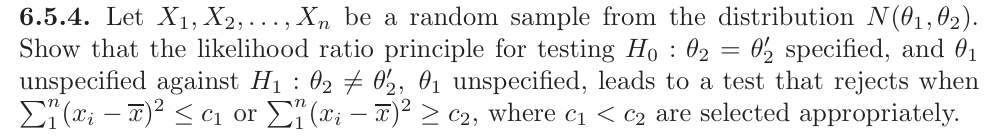
\includegraphics[width=\textwidth]{hw10-2025051117.png}
% \caption{}
\label{}
\end{figure}
\end{exercise}
Consider testing
\[
H_0:\theta\in\Theta_0=\mathbb{R}\times\{ \theta_2' \}\qquad \text{versus}\qquad H_1:\theta \not\in\Theta_0
\]
The likelihood ratio statistic is
\[
\lambda=2\log \left( \frac{\sup_{\theta\in\Theta}L(\theta)}{\sup_{\theta\in\Theta_0}L(\theta)} \right)
\]
where
\[
\begin{aligned}
L(\theta) & =\prod_{i=1}^{n} f(X_i;\theta_1,\theta_2)=\prod_{i=1}^{n} \frac{1}{\sqrt{ 2\pi\theta_2 }}\exp \left\{  -\frac{(X_i-\theta_1)^2}{2\theta_2}  \right\} \\
 & =(2\pi\theta_2)^{-n/2 }\cdot \exp \left\{  -\frac{1}{2\theta_2}\sum_{i=1}^{n} (X_i-\theta_1)^2  \right\}
\end{aligned}
\]
then
\[
l(\theta)=\log(2\pi\theta_2)^{-n/2 }-\frac{1}{2\theta_2}\sum_{i=1}^{n} (X_i-\theta_1)^2
\]
\[
\frac{ \partial l(\theta) }{ \partial \theta_1 } =\frac{1}{\theta_2}\sum_{i=1}^{n} (X_i-\theta_1)=0\implies  \widehat{\theta_1}=\frac{1}{n}\sum_{i=1}^{n} X_i=\overline{X}
\]
\[
\frac{ \partial l(\theta) }{ \partial \theta_2 } =-\frac{n}{2\theta_2}+\frac{1}{2\theta_2^2}\sum_{i=1}^{n} (X_i-\theta_1)^2=0\implies  \widehat{\theta_2}=\frac{1}{n}\sum_{i=1}^{n} (X_i-\overline{X})^2
\]
\[
\begin{aligned}
L(\widehat{\theta}) & =\left[ 2\pi \cdot\frac{1}{n}\sum_{i=1}^{n}(X_i-\overline{X})^2  \right]^{-n/2 }\exp \left\{  -\frac{1}{2\cdot\frac{1}{n}\sum_{i=1}^{n} (X_i-\overline{X})^2}\sum_{i=1}^{n} (X_i-\overline{X})^2  \right\} \\
 & =\left[ 2\pi \cdot\frac{1}{n}\sum_{i=1}^{n}(X_i-\overline{X})^2  \right]^{-n/2 }\cdot \exp \left\{  -\frac{n}{2}  \right\} 
\end{aligned}
\]
\[
L(\widehat{\theta_0})=(2\pi\theta_2')^{-n/2 }\exp \left\{  -\frac{1}{2\theta_2'} \sum_{i=1}^{n}(X_i-\overline{X})^2  \right\}
\]
\[
\begin{aligned}
\lambda & =2\log\left( \frac{L(\widehat{\theta})}{L(\widehat{\theta_0})} \right) \\
 & =2\log\left( \frac{\left[ 2\pi \cdot\frac{1}{n}\sum_{i=1}^{n} (X_i-\overline{X})^2 \right]^{-n/2 }e^{ -n/2  }}{(2\pi\theta_2')^{-n/2 }\exp \left\{  -\frac{1}{2\theta_2'}\sum_{i=1}^{n} (X_i-\overline{X})^2  \right\}} \right) \\
 & =2\log\left( \left[ \frac{1}{n\theta_2'}\sum_{i=1}^{n} (X_i-\overline{X})^2 \right]^{-n/2 }\exp \left\{  -\frac{n}{2}+\frac{1}{2\theta_2'}\sum_{i=1}^{n} (X_i-\overline{X})^2  \right\} \right) \\
 & =-n\log\left( \frac{1}{n\theta_2'} \sum_{i=1}^{n} (X_i-\overline{X})^2 \right)-n+\frac{1}{\theta_2'}\sum_{i=1}^{n} (X_i-\overline{X})^2 \\
 & \eqqcolon -n\log\left( \frac{1}{n\theta_2'}W \right)-n+\frac{1}{\theta_2'}W \\
 & \sim \chi^{2}(1)
\end{aligned}
\]
We reject $H_0$ at level $\alpha$ provided
\begin{equation}
f(W)\coloneqq -n\log\left( \frac{W}{n\theta_2'} \right)-n+\frac{1}{\theta_2'}W\geq \chi^{2}_{\alpha}(1)
\label{bbac55}
\end{equation}

We know that
\[
f'(W)=-\frac{n}{W}+\frac{1}{\theta_2'}\qquad f(0+)=+\infty,\quad f(+\infty)=+\infty
\]
Then $f$ decreases when $W<n\theta_2'$ and increases when $W>n\theta_2'$; $f(n\theta_2')=0$. Thus the solution of \cref{bbac55} gives
\[
W\leq c_1\text{ or }W\geq c_2
\]
for some $c_1,c_2$.

\begin{exercise}
\begin{figure}[H]
\centering
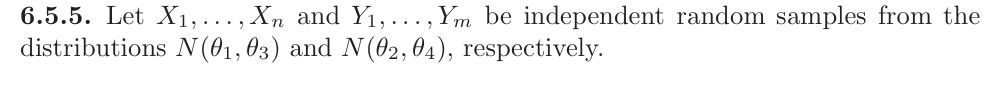
\includegraphics[width=\textwidth]{1-hw10-2025051117.png}
% \caption{}
\label{}
\end{figure}
\begin{figure}[H]
\centering
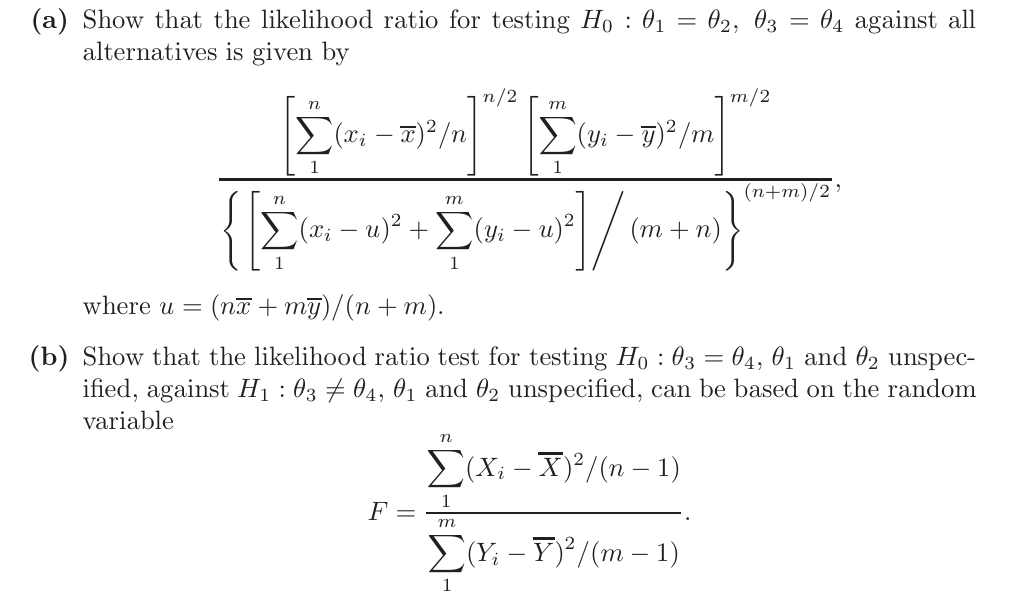
\includegraphics[width=\textwidth]{2-hw10-2025051117.png}
% \caption{}
\label{}
\end{figure}
\end{exercise}
\[
\Theta_0=\{ (\theta_1,\theta_2,\theta_3,\theta_4)\in \mathbb{R}^2\times \mathbb{R}_{>0}^2:\theta_3=\theta_4 \}
\]
The likelihood ratio statistic is
\[
\lambda=2\log \left( \frac{\sup_{\theta\in\Theta}L(\theta)}{\sup_{\theta\in\Theta_0}L(\theta)} \right)
\]
\[
L(\theta)=(2\pi\theta_3)^{-n/2 }\exp \left\{  -\frac{1}{2\theta_3}\sum_{i=1}^{n} (X_i-\theta_1)^2  \right\}\cdot(2\pi\theta_4)^{-m/2 }\exp \left\{  -\frac{1}{2\theta_4}\sum_{j=1}^{m} (Y_j-\theta_2)^2  \right\}
\]
\[
l(\theta)=-\frac{n}{2}\log(2\pi\theta_3)-\frac{m}{2}\log(2\pi\theta_4)-\frac{1}{2\theta_3}\sum_{i=1}^{n} (X_i-\theta_1)^2-\frac{1}{2\theta_4}\sum_{j=1}^{m}(Y_j-\theta_2)^2 
\]
Let $\nabla l(\theta)=0$ then
\[
\widehat{\theta_1}=\overline{X},\quad \widehat{\theta_2}=\overline{Y},\quad \widehat{\theta_3}=\frac{1}{n}\sum_{i=1}^{n} (X_i-\overline{X})^2,\quad \widehat{\theta_4}=\frac{1}{m}\sum_{j=1}^{m} (Y_j-\overline{Y})^2
\]
\[
\sup_{\theta\in\Theta}L(\theta)=\left[ \frac{2\pi}{n}\sum_{i=1}^{n} (X_i-\overline{X})^2 \right]^{-n/2 }\cdot\left[ \frac{2\pi}{m}\sum_{j=1}^{m} (Y_j-\overline{Y})^2 \right]^{-m/2 }\exp \left\{  -\frac{m+n}{2}  \right\}
\]
When $\theta_3=\theta_4$,
\[
\widehat{\theta_3}=\frac{1}{m+n}\left[ \sum_{i=1}^{n} (X_i-\overline{X})^2+\sum_{j=1}^{m} (Y_j-\overline{Y})^2 \right]
\]
\[
\sup_{\theta\in\Theta_0}L(\theta)=\left( \frac{2\pi}{m+n}\left[ \sum_{i=1}^{n} (X_i-\overline{X})^2 +\sum_{j=1}^{m} (Y_j-\overline{Y})^2\right] \right)^{-(m+n)/2 }\exp \left\{  -\frac{m+n}{2}  \right\}
\]
Thus
\[
\begin{aligned}
\lambda & =2\log \left( \frac{\sup_{\theta\in\Theta}L(\theta)}{\sup_{\theta\in\Theta_0}L(\theta)} \right) \\
 & =2\log\left( \frac{\left[ \frac{2\pi}{n}\sum_{i=1}^{n} (X_i-\overline{X})^2 \right]^{-n/2 }\cdot\left[ \frac{2\pi}{m}\sum_{j=1}^{m} (Y_j-\overline{Y})^2 \right]^{-m/2 }\exp \left\{  -\frac{m+n}{2}  \right\}}{\left( \frac{2\pi}{m+n}\left[ \sum_{i=1}^{n} (X_i-\overline{X})^2 +\sum_{j=1}^{m} (Y_j-\overline{Y})^2\right] \right)^{-(m+n)/2 }\exp \left\{  -\frac{m+n}{2}  \right\}} \right) \\
 & =2\log\left( \frac{\left[ \frac{1}{n}\sum_{i=1}^{n} (X_i-\overline{X})^2 \right]^{-n/2 }\cdot\left[ \frac{1}{m}\sum_{j=1}^{m} (Y_j-\overline{Y})^2 \right]^{-m/2 }}{\left( \frac{1}{m+n}\left[ \sum_{i=1}^{n} (X_i-\overline{X})^2 +\sum_{j=1}^{m} (Y_j-\overline{Y})^2\right] \right)^{-(m+n)/2 }} \right)  \\
 & =2\log\left( \frac{\left[ \frac{\sum_{i=1}^{n} (X_i-\overline{X})^2}{\sum_{j=1}^{m} (Y_j-\overline{Y})^2}  \right]^{-n/2 }\cdot n^{\frac{n}{2}}\cdot m^{\frac{m}{2}}}{\left( \left[ \frac{\sum_{i=1}^{n} (X_i-\overline{X})^2}{\sum_{j=1}^{m} (Y_j-\overline{Y})^2}+1\right] \right)^{-(m+n)/2 }\cdot(m+n)^{\frac{m+n}{2}}} \right) \\
 & =2\log\left( \frac{(\frac{n-1}{m-1}F)^{-n/2 }\cdot n^{\frac{n}{2}}\cdot m^{\frac{m}{2}}}{\left( \frac{n-1}{m-1}F \right)^{-(m+n)/2 }\cdot(m+n)^{\frac{m+n}{2}}} \right)
\end{aligned}
\]
So the test can be based on $F$.

\begin{exercise}
\begin{figure}[H]
\centering
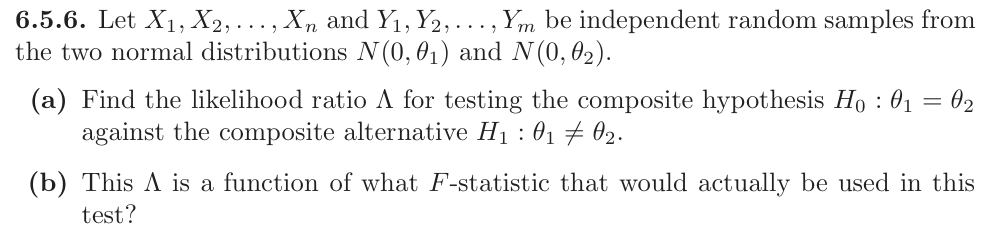
\includegraphics[width=\textwidth]{3-hw10-2025051117.png}
% \caption{}
\label{}
\end{figure}
\end{exercise}
(a)
\[
\Theta_0=\{ (\theta_1,\theta_2)\in \mathbb{R}_{>0}^2:\theta_1=\theta_2 \}
\]
\[
\Lambda=\frac{\sup_{\theta\in\Theta_0}L(\theta)}{\sup_{\theta\in\Theta}L(\theta)}=\frac{\left[ \frac{2\pi}{m+n}\left( \sum_{i=1}^{n} X_i^2+\sum_{j=1}^{m} Y_j^2 \right) \right]^{-\frac{m+n}{2}}}{\left( \frac{2\pi}{n} \sum_{i=1}^{n} X_i^2\right)^{-\frac{n}{2}}\cdot\left( \frac{2\pi}{m}\sum_{j=1}^{m} Y_j^2 \right)^{-\frac{m}{2}}}
\]
(b)
Under $H_0$,
\[
F=\frac{\frac{1}{n}\sum_{i=1}^{n} X_i^2}{\frac{1}{m}\sum_{j=1}^{m}Y_j^2 }\sim F(n,m)
\]
\begin{exercise}
\begin{figure}[H]
\centering
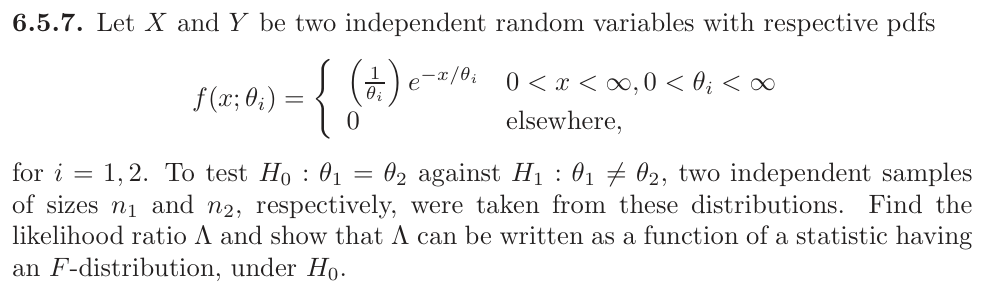
\includegraphics[width=\textwidth]{4-hw10-2025051117.png}
% \caption{}
\label{}
\end{figure}
\end{exercise}
\[
L(\theta)=\theta_1^{-n_1}\theta_2^{-n_2}\exp \left\{  -\frac{1}{\theta_1}\sum_{i=1}^{n_1} X_i-\frac{1}{\theta_2}\sum_{j=1}^{n_2} Y_j  \right\}
\]
\[
\nabla l(\theta)=\left( -\frac{n_1}{\theta_1} +\frac{1}{\theta_1^2}\sum_{i=1}^{n_1} X_i,-\frac{n_2}{\theta_2}+\frac{1}{\theta_2^2}\sum_{j=1}^{n_2} Y_j\right)
\]
Let $\nabla l(\theta)=0$, then
\[
\widehat{\theta_1}=\overline{X},\qquad \widehat{\theta_2}=\overline{Y}
\]
Under $H_0$,
\[
\widehat{\theta_0}=\frac{n_1\overline{X}+n_2\overline{Y}}{n_1+n_2}
\]
Then
\[
\Lambda=\frac{L(\widehat{\theta_0})}{L(\widehat{\theta})}=\frac{(\frac{n_1\overline{X}+n_2\overline{Y}}{n_1+n_2})^{-n_1-n_2}\cdot \exp \{ -n_1-n_2 \}}{\overline{X}^{-n_1}\cdot \overline{Y}^{-n_2}\cdot \exp \{ -n_1-n_2 \}}=\frac{(\frac{n_1\overline{X}+n_2\overline{Y}}{n_1+n_2})^{-n_1-n_2}}{\overline{X}^{-n_1}\cdot \overline{Y}^{-n_2}}
\]
\[
F=\frac{\overline{X}}{\overline{Y}}
\]
\begin{exercise}
\begin{figure}[H]
\centering
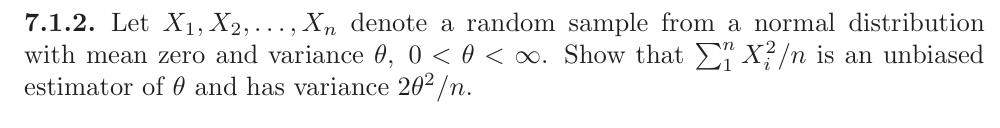
\includegraphics[width=\textwidth]{5-hw10-2025051117.png}
% \caption{}
\label{}
\end{figure}
\end{exercise}
\[
X_i\sim N(0,\theta)\Rightarrow \frac{1}{\sqrt{ \theta }}X_i\sim N(0,1)\Rightarrow\frac{X_i^2}{\theta}\sim \chi^{2}(1)\Rightarrow \mathbb{E}(X_i^2/\theta)=1\Rightarrow \mathbb{E}(X_i^2)=\theta
\]
\[
\mathbb{E}\left( \sum_{i=1}^{n} \frac{X_i^2}{n} \right)=\frac{1}{n}\sum_{i=1}^{n} \mathbb{E}X_i^2=\theta
\]
$\sum_{i=1}^{n}X_i^2/n$ is an unbiased estimator of $\theta$.
\[
\mathrm{Var}\left( \sum_{i=1}^{n} \frac{X_i^2}{n} \right)=\frac{\theta^{2}}{n^2}\sum_{i=1}^{n}\underbrace{ \mathrm{Var}(X_i^2/\theta) }_{ =2 }=\frac{2\theta^{2}}{n}
\]
\begin{exercise}
\begin{figure}[H]
\centering
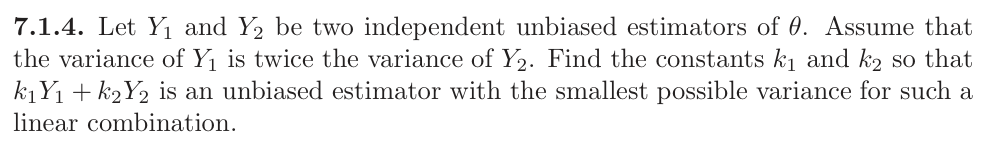
\includegraphics[width=\textwidth]{6-hw10-2025051117.png}
% \caption{}
\label{}
\end{figure}
\end{exercise}
\[
\mathbb{E}[k_1Y_1+k_2Y_2]=(k_1+k_2)\theta=\theta\Rightarrow k_1+k_2=1
\]
\[
\begin{aligned}
\mathrm{Var}(k_1Y_1+k_2Y_2) & =k_1^2\mathrm{Var}(Y_1)+k_2^2\mathrm{Var}(Y_2)=(2k_1^2+k_2^2)\mathrm{Var}(Y_2) \\
 & =\frac{2}{3}\underbrace{ \left( \frac{1}{2}+1 \right)(2k_1^2+k_2^2) }_{ \geq (k_1+k_2)^2 }\mathrm{Var}(Y_2)
\end{aligned}
\]
The equality holds iff
\[
\frac{\sqrt{ 2 }k_1}{1/\sqrt{ 2 }}=k_2\iff k_2=2k_1 \iff k_1=\frac{1}{3},k_2=\frac{2}{3}
\]
\begin{exercise}
\begin{figure}[H]
\centering
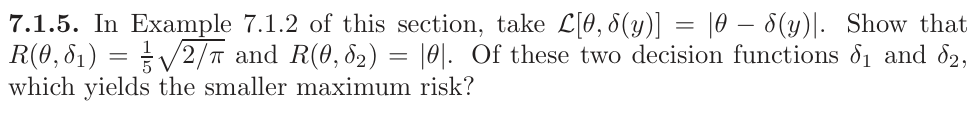
\includegraphics[width=\textwidth]{7-hw10-2025051117.png}
% \caption{}
\label{}
\end{figure}
\end{exercise}
\[
Y=\overline{X}\sim N\left( \theta,\frac{1}{n} \right)
\]
\[
\delta_1(y)=y\qquad \delta_2(y)=0
\]
\[
\begin{aligned}
R(\theta,\delta_1) & =\mathbb{E}\{ \mathcal{L}[\theta,\delta_1(Y)] \}=\mathbb{E}[\lvert \theta-Y \rvert ] \\
 & =\int_{-\infty}^{\infty} \lvert \theta-y \rvert \cdot\frac{1}{\sqrt{ 2\pi/n  }}\exp \left\{ - \frac{1}{2/n }(y-\theta)^2  \right\} \, \mathrm{d}y \\
 & =\sqrt{ \frac{2}{n\pi} }
\end{aligned}
\]
\[
R(\theta,\delta_2)  =\mathbb{E}[\lvert \theta-0 \rvert ]=\lvert \theta \rvert 
\]
When $\lvert \theta \rvert>\sqrt{ \frac{2}{n\pi} }$, $R(\theta,\delta_1)$ is smaller maximum risk; otherwise, $R(\theta,\delta_2)$ is.

\begin{figure}[H]
\centering
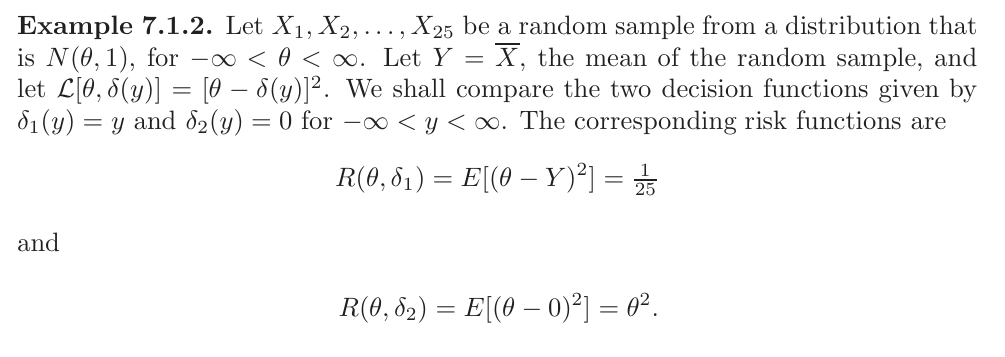
\includegraphics[width=\textwidth]{hw10-2025051120.png}
% \caption{}
\label{}
\end{figure}
\begin{figure}[H]
\centering
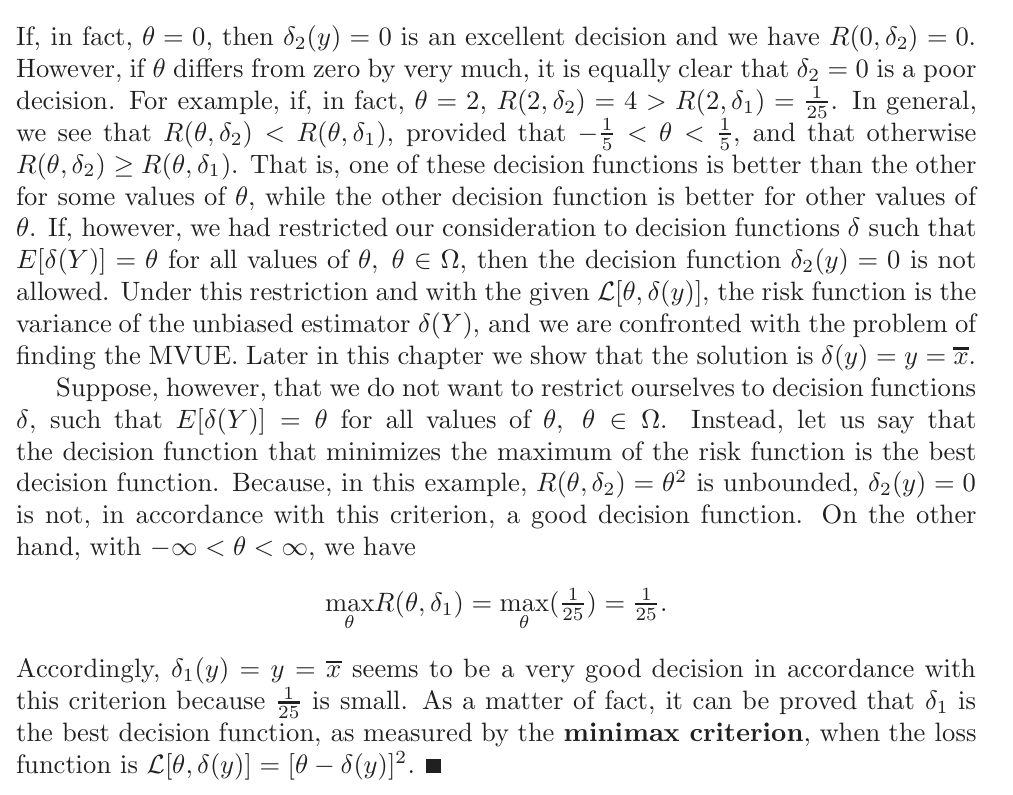
\includegraphics[width=\textwidth]{2-hw10-2025051120.png}
% \caption{}
\label{}
\end{figure}

\begin{exercise}
\begin{figure}[H]
\centering
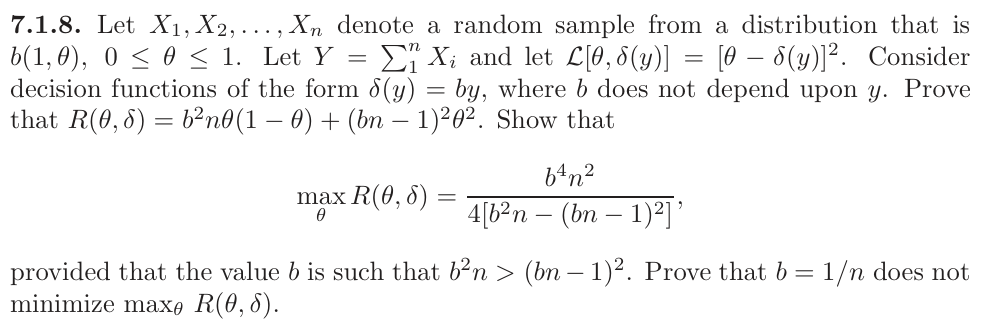
\includegraphics[width=\textwidth]{8-hw10-2025051117.png}
% \caption{}
\label{}
\end{figure}
\end{exercise}
\[
Y=\sum_{i=1}^{n} X_i\sim b(n,\theta)
\]
\[
\begin{aligned}
R(\theta,\delta) & =\mathbb{E}\{ \mathcal{L}[\theta,\delta] \}=\mathbb{E}([\theta-\delta(Y)]^2)=\mathbb{E}[(\theta-bY)^2]  \\
 & =b^2\underbrace{ \mathbb{E}(Y^2) }_{ =n\theta(1-\theta)+(n\theta)^2 }-2b\underbrace{ \mathbb{E}(Y) }_{ =n\theta }+\theta^{2} \\
 & =b^2n\theta(1-\theta )-(bn-1)^2\theta^{2}
\end{aligned}
\]
\[
\frac{ \partial   }{ \partial \theta } R(\theta,\delta)=nb^2-(2nb^2-2n^2b^2+4nb-2)\theta
\]
Let $\frac{ \partial R(\theta,\delta) }{ \partial \theta }=0$, then
\[
\theta=\frac{nb^2/2 }{nb^2-(nb-1)^2}
\]
\[
\max_{\theta}R(\theta,\delta)=R\left( \frac{nb^2/2 }{nb^2-(nb-1)^2},\delta \right)=\frac{n^2b^2}{4[nb^2-(nb-1)^2]}
\]
\[
\begin{aligned}
\frac{ \partial   }{ \partial b }\max_{\theta}R(\theta,\delta) & =\frac{n^2}{4}\cdot\frac{4nb^{5}-4b^3(nb-1)^2-2b^{4}}{[nb^2-(nb-1)^2]^2}  \\
 & \overset{ \text{let }b=\frac{1}{n} }{ = }\frac{n^2}{4}\frac{4n^{-4}-2n^{-4}}{n^{-2}} \\
 & =\frac{1}{2}\neq0 
\end{aligned}
\]
Thus, $b=\frac{1}{n}$ does not minimize $\max_{\theta}R(\theta,\delta)$. (If so, $\frac{\partial}{\partial b}\left.\max_{\theta}R(\theta,\delta)\right|_{b=\frac{1}{n}}=0$, which is a contradiction.)
